%
% This document describes the ee know-how used in Qucs.
%
% Copyright (C) 2003, 2004, 2005, 2006, 2007 Stefan Jahn <stefan@lkcc.org>
% Copyright (C) 2004 Michael Margraf <Michael.Margraf@alumni.TU-Berlin.DE>
%
% Permission is granted to copy, distribute and/or modify this document
% under the terms of the GNU Free Documentation License, Version 1.1
% or any later version published by the Free Software Foundation.
%

\documentclass[10pt,a4paper,oneside]{report}
\usepackage{a4wide}
\usepackage{epsfig}
\usepackage{array}
\usepackage{amsmath}
\usepackage{amsfonts}
\usepackage{stmaryrd}
\usepackage[amssymb]{SIunits}
\usepackage{graphics}
\usepackage{psfrag}
\usepackage{relsize}
\usepackage[section]{placeins}
\usepackage{listings}
\usepackage{longtable}

% Compatibility code for LaTeX and pdfTeX.
%\newif\ifpdf
%\ifx\pdfoutput\undefined
%  \pdffalse
%\else
%  \ifx\pdfoutput\relax
%    \pdffalse
%  \else
%    \ifcase\pdfoutput
%      \pdffalse
%    \else
%      \pdftrue
%    \fi
%  \fi
%\fi

% Only evaluated if run using pdfTeX.
%\ifpdf
\usepackage[pdftex,
	a4paper,
	bookmarks,
	bookmarksopen=true,
	bookmarksnumbered=true,
	pdfpagemode=UseOutlines,
	baseurl=(http://qucs.sourceforge.net),
	pdfstartview=FitH,
	colorlinks,
	linkcolor=black,
	urlcolor=black,
	citecolor=black,
	backref=false,
	plainpages=false,
	pagebackref=false]{hyperref}
\pdfcompresslevel 9
\pdfinfo {
  /Title   (Qucs)
  /Subject (Technical Papers)
  /Author  (Stefan Jahn and Michael Margraf and Vincent Habchi
	and Raimund Jacob)
}
%\fi

% Title page definitions.
\makeatletter
\renewcommand{\maketitle}{\begin{titlepage}%
    \setlength{\parindent}{0pt}
    \vspace*{3cm}
    \begin{flushleft}
      \textbf{\begin{huge}\@title\end{huge}}
    \end{flushleft}
    \hrule height 3pt
    \begin{flushright}
      \begin{LARGE}Technical Papers\end{LARGE}
    \end{flushright}
    \vfill
    \begin{flushright}
      \begin{Large}\@author\end{Large}
    \end{flushright}
    \hrule height 3pt
    \vspace*{24pt}

Copyright \copyright{} 2003, 2004, 2005, 2006, 2007 Stefan Jahn
\textless stefan@lkcc.org\textgreater

Copyright \copyright{} 2003, 2004, 2005, 2006, 2007 Michael Margraf
\textless michael.margraf@alumni.tu-berlin.de\textgreater

Copyright \copyright{} 2004, 2005 Vincent Habchi, F5RCS
\textless 10.50@free.fr\textgreater

Copyright \copyright{} 2005 Raimund Jacob
\textless raimi@lkcc.org\textgreater

    \vspace*{12pt}

Permission is granted to copy, distribute and/or modify this document
under the terms of the GNU Free Documentation License, Version 1.1 or
any later version published by the Free Software Foundation.  A copy
of the license is included in the section entitled "GNU Free
Documentation License".

    \vspace*{1cm}

    \end{titlepage}%
    \setcounter{footnote}{0}%
}
\makeatother

\author{Stefan Jahn\\Michael Margraf\\Vincent Habchi\vspace*{6pt}\\Raimund Jacob}
\title{Qucs}
\date{}

% Here finally starts everything.
\begin{document}

\maketitle

\tableofcontents

\setlength{\parindent}{0pt}
\newpage


\chapter{Introduction}

Qucs consists of two parts: The simulator backend and a frontend, provding a GUI for drawing schematics, controlling simulation, and displaying the simulation results. The operation of the simulation backend is controlled via a text file (called \emph{netlist} in the following) which describes the circuit to be simulated and the simulation(s) to perform in a textual manner. The simulation backend outputs simulation data. This document describes the syntax of netlist files, shows how the netlists are actually used to control Qucs, and finally demonstrates how the simulation data can be visualized via GNU Octave.

Controlling Qucs via netlists and using a separate program for visualizing simulation data may seem complex at first glance; this approach, however, poses the advantage of allowing more flexible usage scenarios: The potentially cpu-consuming circuit simulation could be executed on a powerful (even remote) server, while the result visualization can be done locally on a different computer. By creating netlists via other programs / scripts, it is easy to setup batch simulations.


\section{Outline}

After defining the prerequisites, Chaper \ref{chap:basics} presents a basic example netlist and shows how the simulation data can be visualized in Octave. Chapter \ref{chap:devices} describes the various devices and schematic elements provided by Qucs; Chapter \ref{chap:simulation} describes the simulation commands.


\chapter{Basics}
\label{chap:basics}
\section{Prerequisites}

Qucs installed \verb+qucsator+ command available

The m-files located under \verb+qucs/qucs/octave+.

\begin{verbatim}
Type:Name [node list] [parameters]
\end{verbatim}

Every schematic element has a type and is instantiated with a specific name. 

\chapter{Example}

In this chapter we will start with a simple example of performing an AC simulation of the circuit shown in Fig. \ref{fig:rc_ac_circuit}. 

\begin{figure}[h]
\begin{center}
	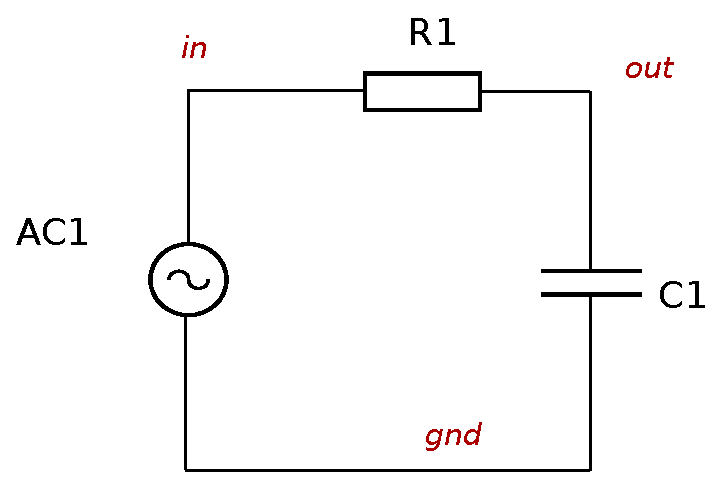
\includegraphics[angle=0,width=0.4\linewidth]{rc_ac_circuit.eps}
	\caption{Circuit}
	\label{fig:rc_ac_circuit}
\end{center}
\end{figure}

The texts in red denote the node names and can be chosen freely. The netlist corresponding to the circuit is shown below.

\begin{verbatim}
Vac:V1 in gnd U="1 V" f="1 kHz"
R:R1 out in R="1 kOhm"
C:C1 out gnd C="10 nF"
\end{verbatim}

It can be seen that the file is structured line-wise; every line instantiates one schematic element. The netlist instantiates

\begin{itemize}
\item a resistor R1 with resistance $R=1\text{k}\Omega$,
\item a capacitor C1 with capacity$C=10$nF, and 
\item an AC source AC1 with "1"V peak-peak voltage(??) and a frequency of $1$kHz.
\end{itemize}

 Storing this netlist in a file \verb+rc_ac.net+ and feeding it into the simulator 

\begin{verbatim}
qucsator < rc_ac.net
\end{verbatim}

yields the following result:

\begin{verbatim}
parsing netlist...
checking netlist...
checker error, no actions defined: nothing to do
\end{verbatim}

Qucs does not know what to do as we did not define any simulations to perform! Deciding to perform an AC sweep, we add the another line to the netlist, yielding:

\begin{verbatim}
Vac:V1 in gnd U="1 V" f="1 kHz"
R:R1 out in R="1 kOhm"
C:C1 out gnd C="10 nF"

.AC:AC1 Type="log" Start="1 Hz" Stop="10 MHz" Points="300" Noise="no"
\end{verbatim}

Using this modified netlist with qucs starts an AC analysis of the circuit. The simulation data is written to stdout; for further processing we save the data in a file called \verb+rc_ac.dat+.

\begin{verbatim}
qucsator < rc_ac.net > rc_ac.dat
\end{verbatim}

Starting GNU Octave and issuing the following commands

\begin{verbatim}
data=loadQucsDataSet('temp.dat')
loglog(data(1).data, data(3).data)
\end{verbatim}

produces a log-log plot of the output voltage versus the frequency. A slightly more polished plot is shown in Fig. \ref{plot:rc_ac}.

\begin{figure}[h]
\begin{center}
	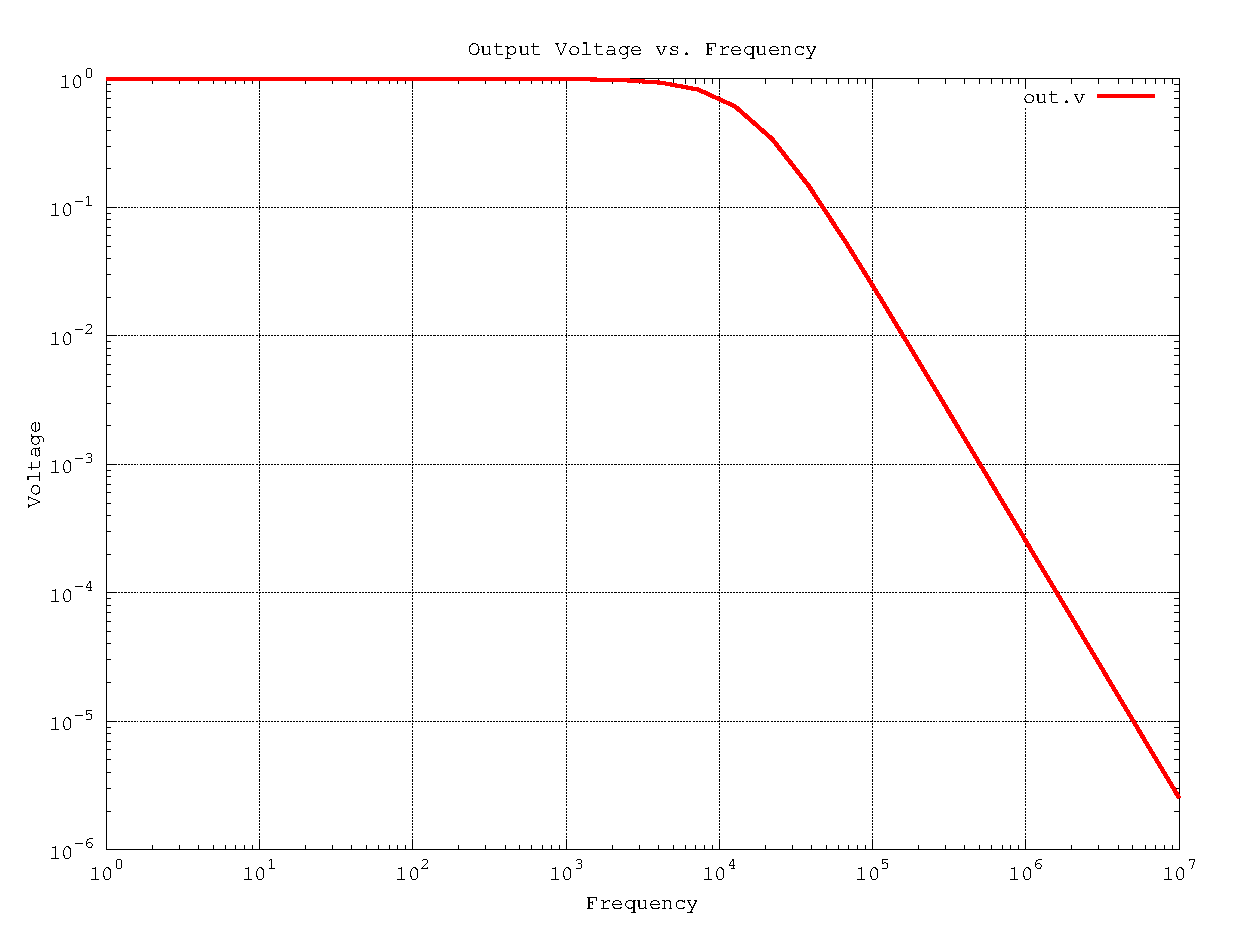
\includegraphics[angle=0,width=0.8\linewidth]{rc_ac.eps}
	\caption{Simulation Result}
	\label{plot:rc_ac}
\end{center}
\end{figure}



\chapter{Qucs Devices}
\label{chap:devices}

\section{Passive Devices}

\subsection{Resistor}

\begin{verbatim}
R:Name Node1 Node2 [Parameters]
\end{verbatim}


\begin{tabular}{|l|p{0.5\linewidth}|l|l|}
\hline
Parameter & Name & Default & Value Mandatory \\
\hline
R & ohmic resistance in Ohms & n/a & yes \\
Temp & simulation temperature in degree Celsius & $26.85$ & no \\
Tc1 & first order temperature coefficient & $0.0$ & no \\
Tc2 & second order temperature coefficient & $0.0$ & no \\
Tnom & temperature at which parameters were extracted & $26.85$ & no \\
\hline
\end{tabular}


\subsection{Capacitor}

\begin{verbatim}
C:Name Node1 Node2 [Parameters]
\end{verbatim}


\begin{tabular}{|l|p{0.5\linewidth}|l|l|}
\hline
Parameter & Name & Default Value & Mandatory \\
\hline
C & capacitance in Farad & n/a & yes \\
V & initial voltage for transient simulation & n/a & no \\
\hline
\end{tabular}


\subsection{Inductor}

\begin{verbatim}
L:Name Node1 Node2 [Parameters]
\end{verbatim}


\begin{tabular}{|l|p{0.5\linewidth}|l|l|}
\hline
Parameter & Name & Default Value & Mandatory \\
\hline
L & inductance in Henry & n/a & yes \\
I & initial current for transient simulation & n/a & no \\
\hline
\end{tabular}


\section{Sources}


\subsection{DC Voltage Source}

\begin{verbatim}
V:Name Node1 Node2 [Parameters]
\end{verbatim}


\begin{tabular}{|l|p{0.5\linewidth}|l|l|}
\hline
Parameter & Name & Default Value & Mandatory \\
\hline
U & voltage in Volts & & yes \\
\hline
\end{tabular}


\subsection{AC Voltage Source}

\begin{verbatim}
Vac:Name Node1 Node2 [Parameters]
\end{verbatim}


\begin{tabular}{|l|p{0.5\linewidth}|l|l|}
\hline
Parameter & Name & Default Value & Mandatory \\
\hline
U & peak voltage in Volts & n/a & yes \\
f & frequency in Hertz & n/a & no \\
Phase & initial phase in degrees & 0 & no \\
Theta & damping factor (transient simulation only) & 0 & no \\
\hline
\end{tabular}


%& & & \\

\chapter{Simulation Commands}
\label{chap:simulation}


\section{DC Simulation}


\begin{verbatim}
.DC:Name [Parameters]
\end{verbatim}


\begin{tabular}{|l|p{0.5\linewidth}|l|l|}
\hline
Parameter & Name & Default Value & Mandatory \\
\hline
Temp & simulation temperature in degree Celsius& $26.85$ & no \\
reltol & relative tolerance for convergence & 0.001 & no \\
absol & absolute tolerance for currents & 1 pA & no \\
vntol & absolute tolerance for voltages & 1 uV & no \\
saveOPs & put operating points into dataset [yes,no]& & no \\
MaxIter & maximum number of iterations until error & 150 & no \\
saveAll & save subcircuit nodes into dataset [yes,no]& no & no\\
convHelper & preferred convergence algorithm [none, gMinStepping, SteepestDescent, LineSearch, Attenuation, SourceStepping]& none & \\
Solver & method for solving the circuit matrix [CroutLU, DoolittleLU, HouseholderQR, HouseholderLQ, GolubSVD] & CroutLU & no \\
\hline
\end{tabular}


\section{AC Simulation}


\begin{verbatim}
.AC:Name [Parameters]
\end{verbatim}


\begin{tabular}{|l|p{0.5\linewidth}|l|l|}
\hline
Parameter & Name & Default Value & Mandatory \\
\hline
Type & sweep type [lin,log,list,const] & n/a & yes \\
Start & start frequency in Hertz & n/a & yes \\
Stop & stop frequency in Hertz & n/a & yes \\
Points & number of simulation steps & n/a & yes \\
Noise & calculate noise voltages & no & no \\
\hline
\end{tabular}



\section{Parameter Sweep}


\begin{verbatim}
.SW:Name [Parameters]
\end{verbatim}


\begin{tabular}{|l|p{0.5\linewidth}|l|l|}
\hline
Parameter & Name & Default Value & Mandatory \\
\hline
Sim & simulation to perform parameter sweep on & n/a & yes \\
Type & sweep type [lin,log,list,const] & n/a & yes \\
Param & parameter to sweep & n/a & yes \\
Stop & start value for sweep & n/a & yes \\
Start & stop value for sweep & n/a & yes \\
\hline
\end{tabular}



\section{Transient Simulation}


\begin{verbatim}
.TR:Name [Parameters]
\end{verbatim}


\begin{tabular}{|l|p{0.5\linewidth}|l|l|}
\hline
Parameter & Name & Default Value & Mandatory \\
\hline
Type & sweep type [lin,log,list,const] & todo & todo \\
Start & start time in seconds & todo & todo \\
Stop & stop time in seconds & todo & todo \\
Points & number of simulation time steps & 11(todo) & todo \\
IntegrationMethod & integration method [Euler, Trapezoidal, Gear, AdamsMoulton] & Trapezoidal & todo \\
Order & order of integration method & 2 & todo \\
InitialStep & initial step size in seconds & 1 ns (todo) & todo \\
MinStep & minimum step size in seconds & 1e-16 & todo \\
MaxIter & maximum number of iterations until error & 150 & todo \\
reltol & relative tolerance for convergence & 0.001 & todo \\
abstol & absolute tolerance for currents & 1 pA & todo \\
vntol & absolute tolerance for voltages & 1 uV & todo \\
Temp & simulation temperature in degree Celsius & 26.85 & todo \\
LTEreltol & relative tolerance of local truncation error & 1e-3 & todo \\
LTEabstol & absolute tolerance of local truncation error & 1e-6 & todo \\
LTEfactor & overestimation of local truncation error & 1 & todo \\
Solver & method for solving the circuit matrix [CroutLU, DoolittleLU, HouseholderQR, HouseholderLQ, GolubSVD] & CroutLU & todo \\
relaxTSR & relax time step raster [no, yes] & yes & todo \\
initialDC & perform an initial DC analysis [yes, no] & yes & todo \\
MaxStep & maximum step size in seconds & 0 & todo \\
\hline
\end{tabular}

%& & & \\



\end{document}
